\chapter{Implementazioni future}

Considerando i componenti mancanti, le funzionalità che vorremmo
implementare in un prossimo futuro sono le seguenti:

\begin{itemize}
\item Interfaccia utente attraverso il display \textit{OLED}
\item Sensing di tensione e corrente prodotti dal pannello
\item Struttura per pannello, motori e sensori
\item Interfaccia \textit{Python} via \textit{COM} port con visualizzazione valori, statistiche e controllo manuale motori
\end{itemize}

\noindent L'interfaccia utente nel display OLED mostrerà: tensione e
corrente del pannello, posizione del sole e posizione pannello (angolo di
Azimuth e angolo di Elevazione), orario e posizione geografica.

\begin{center}
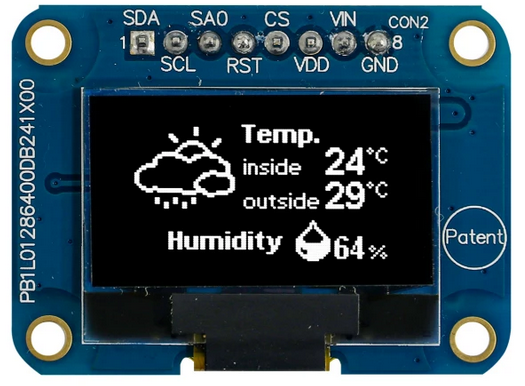
\includegraphics[width=0.4\textwidth]{figures/image27.png}
\captionsetup{type=figure}
\captionof{figure}{Esempio di interfaccia utente su display OLED}
\end{center}

\noindent La struttura di supporto per il pannello servirà prima di tutto a
consentire al pannello di muoversi nei due gradi di libertà (rotazione
intorno all'asse Z e rotazione intorno all'asse Y) e poi per contenere
magnetometro ed accelerometro in modo che questi rilevino esattamente la
posizione del pannello (dovranno quindi essere fisicamente attaccati al
pannello e dovranno muoversi con esso).

\begin{center}
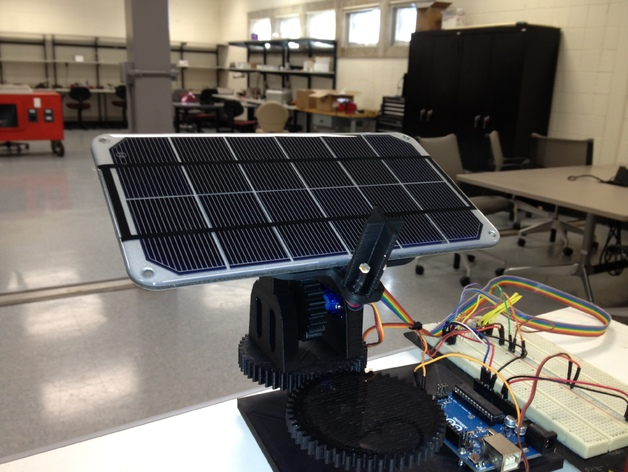
\includegraphics[width=3.63in,height=2.72in]{figures/image52.png}
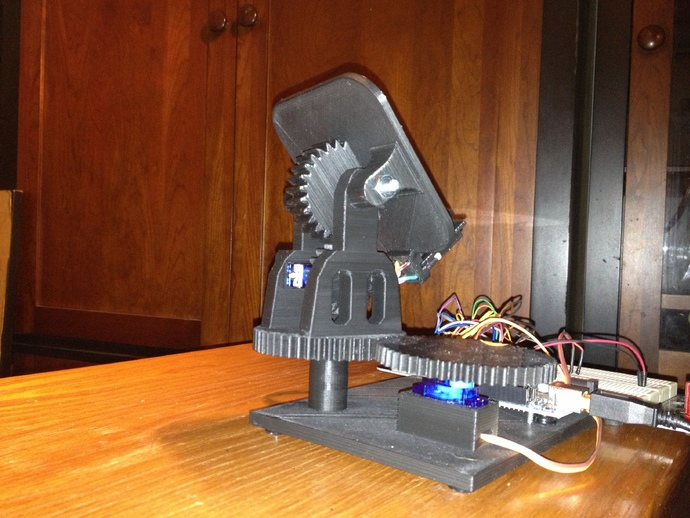
\includegraphics[width=3.63in,height=2.72in]{figures/image68.png}
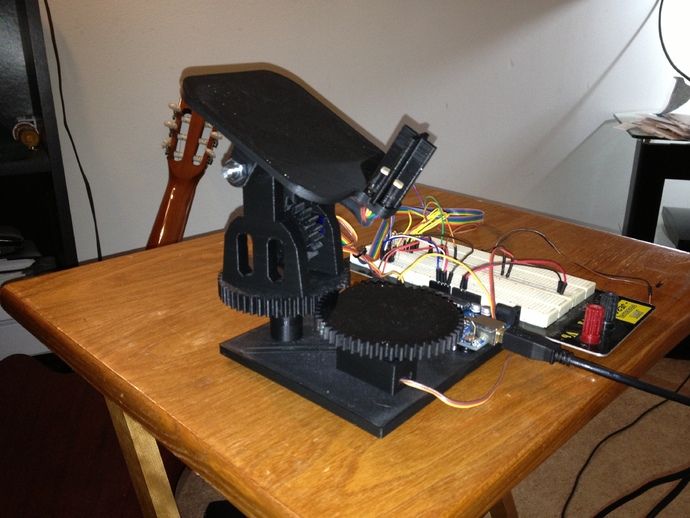
\includegraphics[width=3.63in,height=2.72in]{figures/image20.png}
\captionsetup{type=figure}
\captionof{figure}{Esempio di struttura di supporto per pannello e motori di tipo servo\\
(Credits:\href{https://www.thingiverse.com/thing:53321}{\underline{https://www.thingiverse.com/thing:53321}})}
\end{center}

\noindent Per quanto riguarda l'interfaccia grafica per la connessione seriale via
USB, si pensava di sviluppare in \textit{GUI} (Graphical User Interface) in
linguaggio \textit{Python} che consentisse di controllare manualmente le
posizioni dei motori, di abilitare il tracking o il return to home e
che, attraverso l'uso di piccoli grafici, mostrasse delle semplici
statistiche sulla potenza e l'energia prodotte dal pannello
fotovoltaico.

\begin{center}
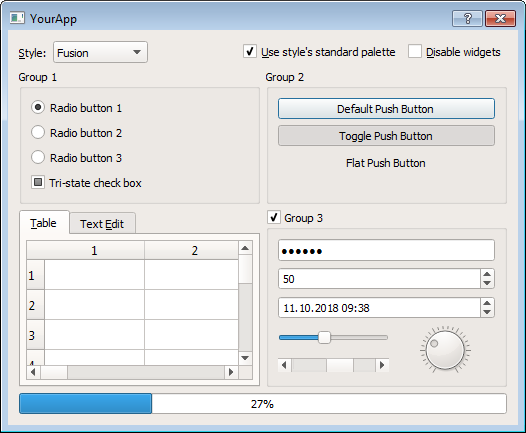
\includegraphics[width=4.68229in,height=3.4426in]{figures/image47.png}
\captionsetup{type=figure}
\captionof{figure}{Esempio di GUI sviluppata in python}
\end{center}

